\newpage
\section{Describing dynamic behaviour with SDMs}

After creating the classdiagrams, normally you would begin now tiping the code for the method implementations. But Moflon offers you the possibility to generate the code automatically. You only have to describe the behaviour in diagrams. We name these diagram types \texttt{Story Driven Modeling (SDM)}. This is a cool and easy way to describe method behaviours.
\newline
For an example we chose a little method, which initializes our Box class. But now lets see how this looks like.

%---------------------------------------------------------------------------------------------------

\subsection{Implementation of the initializeBox method}

\begin{itemize}
\item Open the \texttt{initializeBox Story Diagram} under \texttt{Learning\-Box\-Lan\-guage/Box/initialize\-Box()} (Fig.~\ref{open_deleteNode}).
\end{itemize}
\begin{figure}[htbp]
	\centering
  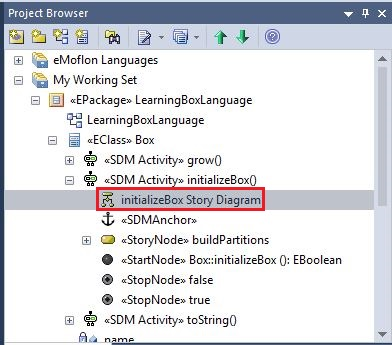
\includegraphics[width=0.6\textwidth]{select_SDM}
	\caption{Open initializeBox Story Diagram} 
	\label{open_deleteNode} 
\end{figure}

In Fig.~\ref{sdm_initializeBox} you see the SDM, which describes the whole function of the \texttt{initializeBox} method. In this method we want to initialize box with two partitions.
\newline
In SDMs a red element will be deleted in the method, a green one created. Black elements still consists. With this knowledge you can easily understand what is going on in this diagram.
\newline
In detail when initializeBox is called two, partitions are created. These are the two green boxes \texttt{firstPartition} and \texttt{lastPartition}. Additional several links are created to link the new elements between each other and to box.
\newline
The crossed out partition \texttt{onePartiton} ensures that box does not contain any partition when initializeBox is called.
\newline
Finally because initializeBox returns an EBoolean value, the return values has to be defined. This is done by the stop nodes. If the above described process was succesful, \texttt{true} will be returned, otherwise \texttt{false}.
\newline
For further information please refer to Part III of the handbook. There everything is explained in detail. But here you can see to describe a whole method is really easy.

\begin{figure}[htbp]
	\centering
  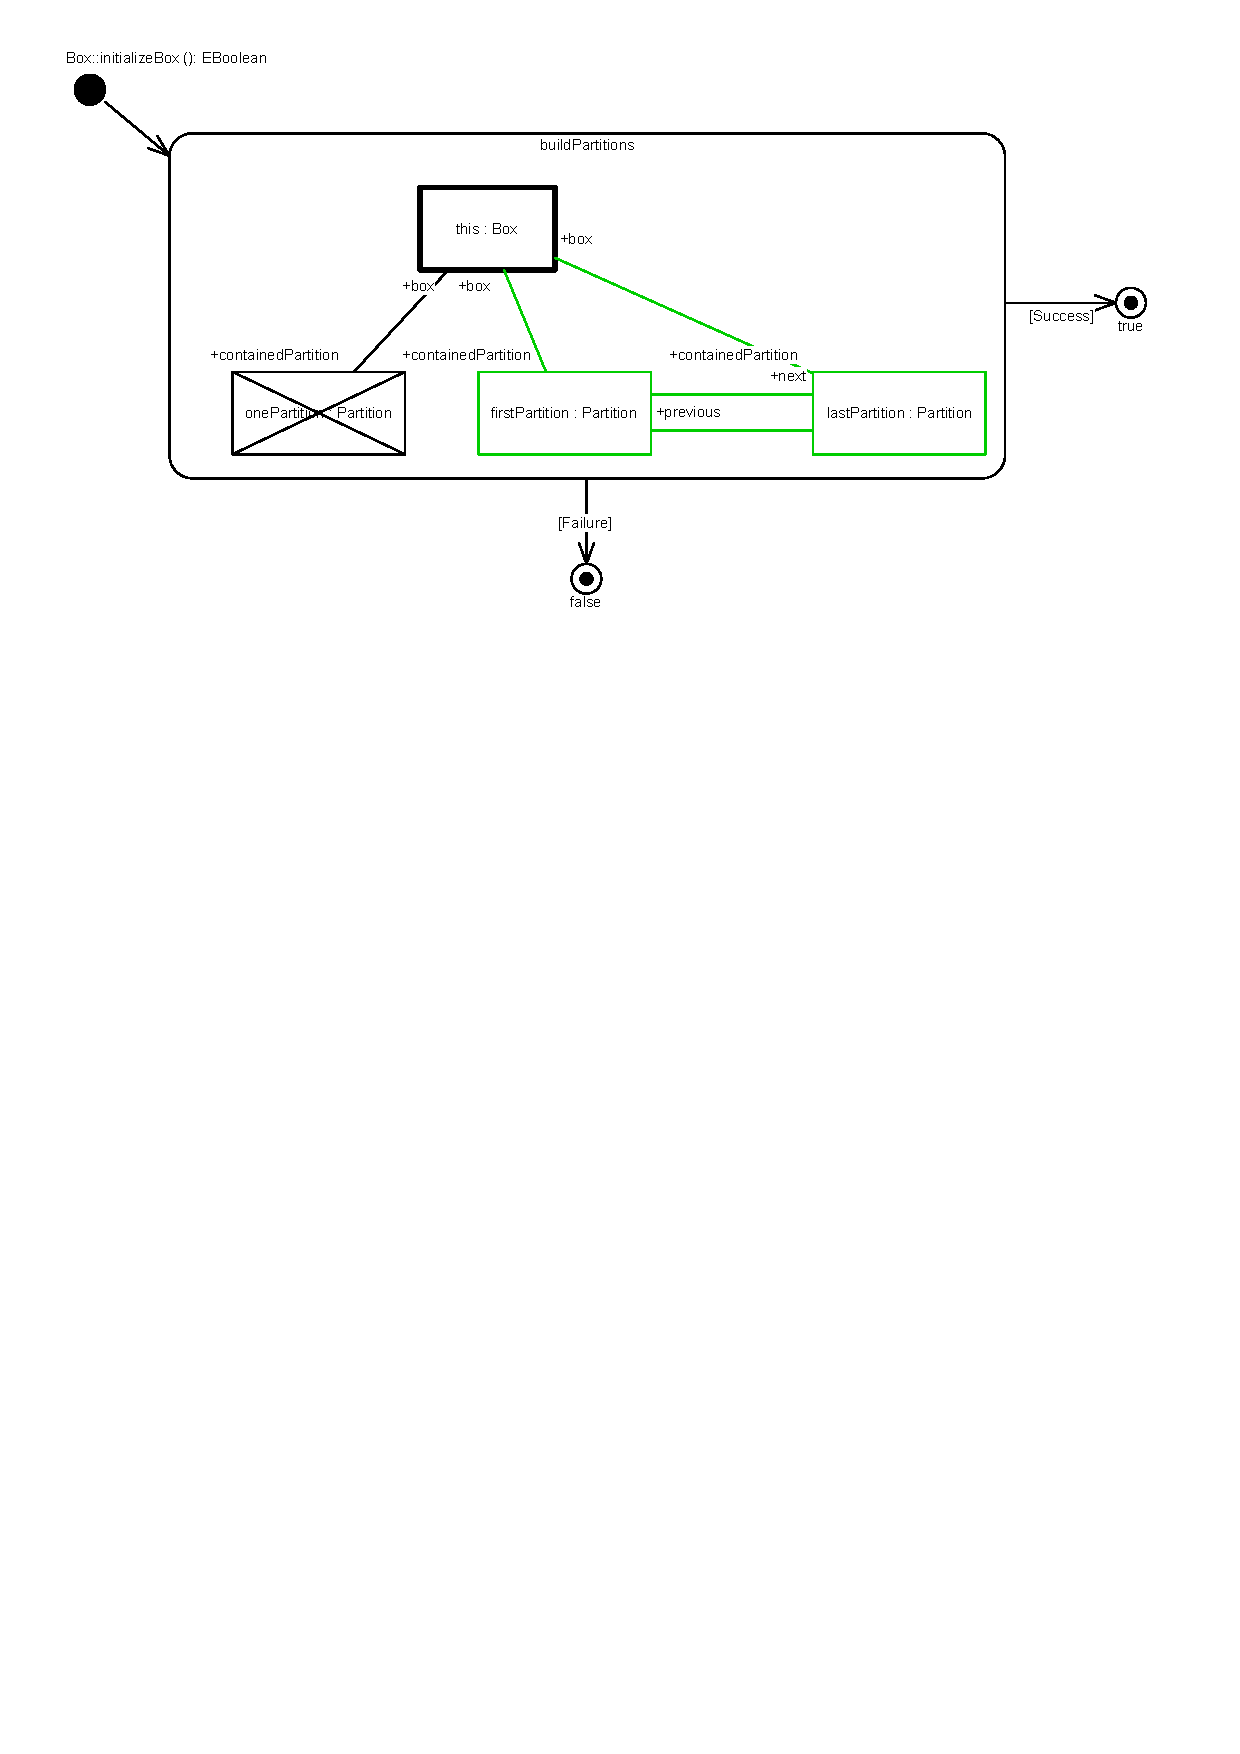
\includegraphics[width=1.2\textwidth]{SDM_initializeBox}
	\caption{initializeBox SDM} 
	\label{sdm_initializeBox} 
\end{figure}



